%%%%%%%%%%%%%%%%%%%%%%%%%%%%%%%%%%%%%%%%%%%%%%%
%
% Template per Elaborato di Laurea
% DISI - Dipartimento di Ingegneria e Scienza dell’Informazione
%
% update 2015-09-10
%
% Per la generazione corretta del 
% pdflatex nome_file.tex
% bibtex nome_file.aux
% pdflatex nome_file.tex
% pdflatex nome_file.tex
%
%%%%%%%%%%%%%%%%%%%%%%%%%%%%%%%%%%%%%%%%%%%%%%%

% formato FRONTE RETRO
\documentclass[epsfig,a4paper,11pt,titlepage,twoside,openany]{book}
\usepackage{epsfig}
\usepackage{plain}
\usepackage{setspace}
\usepackage[paperheight=29.7cm,paperwidth=21cm,outer=1.5cm,inner=2.5cm,top=2cm,bottom=2cm]{geometry} % per definizione layout
\usepackage{titlesec} % per formato custom dei titoli dei capitoli
\usepackage{cancel}
\usepackage{amsmath}
\usepackage{graphicx}
\usepackage{subcaption}
%\usepackage{hyperref}

\usepackage[a-1b]{pdfx}
\usepackage[pdfa]{hyperref}

\renewcommand{\chapterautorefname}{Capitolo}
\usepackage{url}
\usepackage{caption}
\usepackage{booktabs}
\usepackage{tabularx}
\usepackage{makecell}
\usepackage{multirow}
\usepackage{algorithm}
\usepackage{algpseudocode}


\graphicspath{ {./images/} }
%%%%%%%%%%%%%%
% supporto lettere accentate
%
%\usepackage[latin1]{inputenc} % per Windows;
\usepackage[utf8x]{inputenc} % per Linux (richiede il pacchetto unicode);
%\usepackage[applemac]{inputenc} % per Mac.

\singlespacing

\usepackage[italian]{babel}



\usepackage{listings}
\usepackage{color}

\definecolor{dkgreen}{rgb}{0,0.6,0}
\definecolor{gray}{rgb}{0.5,0.5,0.5}
\definecolor{mauve}{rgb}{0.58,0,0.82}

\lstset{frame=tb,
  language=Java,
  aboveskip=3mm,
  belowskip=3mm,
  showstringspaces=false,
  columns=flexible,
  basicstyle={\small\ttfamily},
  numbers=none,
  numberstyle=\tiny\color{gray},
  keywordstyle=\color{blue},
  commentstyle=\color{dkgreen},
  stringstyle=\color{mauve},
  breaklines=true,
  breakatwhitespace=true,
  tabsize=3
}

\begin{document}

  % nessuna numerazione
  \pagenumbering{gobble} 
  \pagestyle{plain}

\thispagestyle{empty}

\begin{center}
  \begin{figure}[h!]
    \centerline{
\psfig{file=logo_unitn_black_center.eps,width=0.6\textwidth}}
  \end{figure}

  \vspace{2 cm} 

  \LARGE{Dipartimento di Ingegneria e Scienza dell’Informazione\\}

  \vspace{1 cm} 
  \Large{Corso di Laurea in\\
    Informatica
    %Ingegneria dell'Informazione e delle Comunicazioni
    %Ingegneria dell'Informazione e Organizzazione d'Impresa
    %Ingegneria Elettronica e delle Telecomunicazioni
  }

  \vspace{2 cm} 
  \Large\textsc{Elaborato finale\\} 
  \vspace{1 cm} 
  \Huge\textsc{Titolo\\}
  \Large{\it{Sottotitolo (alcune volte lungo - opzionale)}}


  \vspace{2 cm} 
  \begin{tabular*}{\textwidth}{ c @{\extracolsep{\fill}} c }
  \Large{Supervisore} & \Large{Laureando}\\
  \Large{Prof. Alberto Montresor}& \Large{Alberto Giust}\\
  \end{tabular*}

  \vspace{2 cm} 

  \Large{Anno accademico 2018/2019}
  
\end{center}



  \clearpage
 
%%%%%%%%%%%%%%%%%%%%%%%%%%%%%%%%%%%%%%%%%%%%%%%%%%%%%%%%%%%%%%%%%%%%%%%%%%
%%%%%%%%%%%%%%%%%%%%%%%%%%%%%%%%%%%%%%%%%%%%%%%%%%%%%%%%%%%%%%%%%%%%%%%%%%
%% Nota
%%%%%%%%%%%%%%%%%%%%%%%%%%%%%%%%%%%%%%%%%%%%%%%%%%%%%%%%%%%%%%%%%%%%%%%%%%
%% Sezione Ringraziamenti opzionale
%%%%%%%%%%%%%%%%%%%%%%%%%%%%%%%%%%%%%%%%%%%%%%%%%%%%%%%%%%%%%%%%%%%%%%%%%%
%%%%%%%%%%%%%%%%%%%%%%%%%%%%%%%%%%%%%%%%%%%%%%%%%%%%%%%%%%%%%%%%%%%%%%%%%%
  \thispagestyle{empty}

\begin{center}
  {\bf \Huge Ringraziamenti}
\end{center}

\vspace{4cm}


\emph{
  Ringrazio la mia famiglia, che mi ha supportato in questi tre anni.
}

  \clearpage
  \pagestyle{plain} % nessuna intestazione e pie pagina con numero al centro

  
  % inizio numerazione pagine in numeri arabi
  \mainmatter

%%%%%%%%%%%%%%%%%%%%%%%%%%%%%%%%%%%%%%%%%%%%%%%%%%%%%%%%%%%%%%%%%%%%%%%%%%
%%%%%%%%%%%%%%%%%%%%%%%%%%%%%%%%%%%%%%%%%%%%%%%%%%%%%%%%%%%%%%%%%%%%%%%%%%
%% Nota
%%%%%%%%%%%%%%%%%%%%%%%%%%%%%%%%%%%%%%%%%%%%%%%%%%%%%%%%%%%%%%%%%%%%%%%%%%
%% Si ricorda che il numero massimo di facciate è 30.
%% Nel conteggio delle facciate sono incluse 
%%   indice
%%   sommario
%%   capitoli
%% Dal conteggio delle facciate sono escluse
%%   frontespizio
%%   ringraziamenti
%%   allegati    
%%%%%%%%%%%%%%%%%%%%%%%%%%%%%%%%%%%%%%%%%%%%%%%%%%%%%%%%%%%%%%%%%%%%%%%%%%
%%%%%%%%%%%%%%%%%%%%%%%%%%%%%%%%%%%%%%%%%%%%%%%%%%%%%%%%%%%%%%%%%%%%%%%%%%

    % indice
    \tableofcontents
    \clearpage
    
    
          
    % gruppo per definizone di successione capitoli senza interruzione di pagina
    \begingroup
      % nessuna interruzione di pagina tra capitoli
      % ridefinizione dei comandi di clear page
      \renewcommand{\cleardoublepage}{} 
      \renewcommand{\clearpage}{} 
      % redefinizione del formato del titolo del capitolo
      % da formato
      %   Capitolo X
      %   Titolo capitolo
      % a formato
      %   X   Titolo capitolo
      
      \titleformat{\chapter}
        {\normalfont\Huge\bfseries}{\thechapter}{1em}{}
        
      \titlespacing*{\chapter}{0pt}{0.59in}{0.02in}
      \titlespacing*{\section}{0pt}{0.20in}{0.02in}
      \titlespacing*{\subsection}{0pt}{0.10in}{0.02in}
      
      % sommario
      \chapter*{Sommario} % senza numerazione
\label{sommario}

\addcontentsline{toc}{chapter}{Sommario} % da aggiungere comunque all'indice

Nel 2010, grazie alla riforma Gelmini \cite{riforma}, la struttura degli istituti superiori ha subito cambiamenti ed alcuni nuovi indirizzi sono stati aggiunti: tra questi il liceo Scientifico - opzione Scienze Applicate in sostituzione del liceo Scientifico PNI. In questo istituto la legge si pone l'obiettivo di dare più importanza all'informatica, ponendo maggiore attenzione sulle potenzialità di questa materia anche come supporto per lo studio di altre materie, in ambito scientifico, ma anche umanistico. Sono passati nove anni dall'approvazione del decreto e dall'introduzione di questo indirizzo negli istituti superiori, ma alcune linee guida sono ancora di difficile attuazione specialmente per mancanza di docenti tecnici di supporto durante le esercitazioni e per il mancato adeguamento alle nuove tecnologie. 

L'acronimo STEM nasce nel 2001 negli Stati Uniti, indica un percorso di studi incentrato su Scienze, Tecnologia, Ingegneria e Matematica, che ha come obiettivo quello di integrare queste materie in un sistema di apprendimento attivo basato su un continuo confronto con applicazioni reali \cite{stem_education}. 

L'aggiunta dell'arte all'interno di questo curriculum, con il relativo cambio di nome da STEM a STEAM, si poggia su un semplice concetto: gli studenti, per avere successo nel mondo del lavoro e della ricerca, devono essere sia metodici e competenti, ma allo stesso tempo devono sfruttare la propria creatività ed il pensiero critico. 

L'ultimo passo, che porta alla nascita di Computational STEAM, viene eseguito integrando l'informatica, già presente all'interno della macro area Tecnologia, non solo come materia a sè stante, ma anche come supporto per le altre discipline. La scienza computazionale sfrutta infatti le potenzialità computazionali dell'informatica per analizzare, organizzare ed elaborare grandi quantità di dati.

Il Dipartimento di Ingegneria e Scienze dell'Informazione (DISI), propone un percorso di studio indirizzato a studenti del liceo Scientifico, chiamato Computational STEAM, con lo scopo di rafforzare le competenze di informatica, integrando questa materia con le altre discipline scientifiche, per offrire agli studenti gli strumenti necessari per capire e toccare con mano come queste ultime si stanno sviluppando nel mondo del lavoro e della ricerca, senza però tralasciare le materie umanistiche, indispensabili per sviluppare un pensiero critico.

Le tematiche affrontate non sono inserite in percorsi specializzanti, ma di più ampio respiro in modo da offrire le basi agli studenti, rimandando poi gli approfondimenti agli studi universitari (seguendo lo spirito generalista che contraddistingue i licei). Durante le ore dedicate all'informatica viene dato spazio ad argomenti quali Data Science e Intelligenza Artificiale, indispensabili oggigiorno sia nel mondo del lavoro che in quello della ricerca sia se si intende proseguire la propria formazione in facoltà di Ingegneria, ma anche in settori quali matematica, fisica, biologia, \dots

Il punto cardine del percorso di studi Computational STEAM rimane comunque quello di formare uno studente in grado di utilizzare l'informatica in ambienti fortemente interdisciplinari. Le potenzialità sono molteplici: dall'analisi di dati in scienze, matematica e fisica alla creazione di simulazione di ambienti reali quali la diffusione delle epidemie o lo studio del volo degli uccelli fino ad arrivare agli studi dell'arte orientale con i suoi pattern regolari che si poggiano su regole matematiche.

L'esperienza di tirocinio, svolta tra i mesi di aprile e maggio presso il Liceo Galileo Galilei (Trento), il liceo Leonardo Da Vinci (Trento), l’istituto tecnico tecnologico Buonarroti-Pozzo (Trento) e il liceo Scientifico presso il collegio Arcivescovile Celestino Endrici (Trento) è stato un primo test per capire se e come questo percorso di studi potesse essere introdotto ai ragazzi. 
Lo stage è stato organizzato da tre studenti ed ognuno ha scelto un argomento diverso tra quelli riportati sopra (più precisamente lo studio delle epidemie e l'utilizzo dei modelli per la comunicazione in sistemi distribuiti, un approfondimento sui frattali e l'analisi di modelli di simulazione ad agente per osservare il comportamento delle formiche ed il volo degli uccelli), seguendo i principi proposti da Computational STEAM quali apprendimento attivo, lavoro in gruppo e risoluzione di problemi (problem solving). Nello specifico questo elaborato riporta un'analisi del modulo proposto riguardante i protocolli epidemici, organizzato su sette ore e presentato in tre classi, di cui due del liceo Scientifico e una dell'istituto tecnico. L'argomento è stato scelto per diverse ragioni: in primo luogo, riesce ad esprimere l'interdisciplinarietà dell'informatica, caratteristica fondamentale per dare uno spunto di riflessione ai ragazzi sulle potenzialità della materia. Infatti, i modelli utilizzati in epidemiologia (il modello SI ed il modello SIR), sono stati adattati e rielaborati per sviluppare alcuni dei protocolli per la distribuzione delle informazioni in sistemi distribuiti.

Inoltre gli algoritmi si basano su regole semplici, adatte ad essere comprese dai ragazzi dal terzo anno in poi, ma che allo stesso tempo possono essere approfondite in modo da risolvere problemi complessi. 

L'elaborato è suddiviso in tre capitoli: Computational STEAM, Protocolli epidemici nel dettaglio e Relazione di tirocinio. Nel primo vengono esposte le motivazione che hanno portato alla proposta di questo nuovo percorso di studi indirizzato ai licei, con un'analisi delle problematiche che rallentano il processo di adeguamento alla riforma ed una serie di proposte per la sua attuazione nei prossimi anni. 

Il secondo capitolo espone nel dettaglio l'argomento tecnico affrontato durante il corso, con ulteriori approfondimenti non trattati durante le ore scolastiche. Durante queste ultime infatti, sono stati presentati i due principali modelli, SI e SIR, con i relativi algoritmi e stili. Gli studenti hanno avuto la possibilità di implementarli su schermo utilizzando l'ambiente di sviluppo Processing e sfruttando una libreria con le classi necessarie per completare gli esercizi proposti. La libreria è stata fornita ad inizio corso, con la relativa documentazione da cui i ragazzi hanno potuto comprenderne il funzionamento. Il secondo capitolo espone anche ulteriori utilizzi dei protocolli epidemici rispetto la disseminazione di informazioni, quali Aggregazione, Peer Sampling e rilevamento di fallimenti all'interno della rete. L'argomento è analizzato dal punto di vista tecnico esponendo le differenze e un'analisi della complessità degli algoritmi.

Il terzo capitolo consiste in una descrizione dell'attività svolta presso gli istituti, l'organizzazione del corso ed il metodo esecutivo seguito. I ragazzi hanno compilato due questionari, creati utilizzando i Moduli Google: uno iniziale per una raccolta di pareri riguardo il loro modo di concepire l'informatica, come questa venga insegnata in classe e per capire il loro livello di conoscenze riguardo l'argomento presentato durante le lezioni successive. Il questionario finale è stato invece utilizzato per raccogliere i pareri dell'esperienza e per capire se gli studenti hanno notato alcune differenze rispetto al metodo di insegnamento "classico". È presente inoltre una descrizione della libreria, scritta in Java, utilizzata per astrarre alcuni concetti non studiati dai ragazzi e per gestire la componente di visualizzazione, necessaria per la generazione di un output accattivante e significativo. I ragazzi hanno avuto la possibilità di visualizzarla, di compilarla e di utilizzare la propria versione oppure di scaricare una versione già precompilata fornita ad inizio del corso. Infine è presente l'analisi dei risultati ottenuti durante l'esperienza di tirocinio con relativi commenti ed opinioni, per un'eventuale riproposta del modulo, o della sua integrazione all'interno di un corso di studi più ampio, come quello di Computational STEAM.

L'esperienza nel complesso è sicuramente positiva e, nonostante il tempo limitato, gli argomenti sono stati trattati in maniera esaustiva. I ragazzi sono rimasti soddisfatti e, da quanto riportato, le tematiche sono state esposte in modo chiaro. Alcuni hanno lamentato un mancato approfondimento ulteriore riguardo il linguaggio di programmazione, che per mancanza di tempo non è avvenuta. 

La scelta dell'utilizzo di Processing, nonostante gli studenti non l'avessero mai utilizzato, si è rivelata comunque utile dal punto di vista dell'efficacia di visualizzazione: ai ragazzi è servito per mantenere alta l'attenzione e l'interesse. 

Gli esercizi proposti non hanno creato molti problemi, perchè alcuni sono stati presentati in modo abbastanza guidato, in modo da prendere confidenza con l'ambiente di sviluppo.
%%%%%%%%%%%%%%%%%%%%%%%%%%%%%%%%%%%%%%%%%%%%%%%%%%%%%%%%%%%%%%%%%%%%%%%%%%
%%%%%%%%%%%%%%%%%%%%%%%%%%%%%%%%%%%%%%%%%%%%%%%%%%%%%%%%%%%%%%%%%%%%%%%%%%
%% Nota
%%%%%%%%%%%%%%%%%%%%%%%%%%%%%%%%%%%%%%%%%%%%%%%%%%%%%%%%%%%%%%%%%%%%%%%%%%
%% Sommario è un breve riassunto del lavoro svolto dove si descrive 
%% l’obiettivo, l’oggetto della tesi, le metodologie e 
%% le tecniche usate, i dati elaborati e la spiegazione delle conclusioni 
%% alle quali siete arrivati.
%% Il sommario dell’elaborato consiste al massimo di 3 pagine e deve contenere le seguenti informazioni: 
%%   contesto e motivazioni
%%   breve riassunto del problema affrontato
%%   tecniche utilizzate e/o sviluppate
%%   risultati raggiunti, sottolineando il contributo personale del laureando/a
%%%%%%%%%%%%%%%%%%%%%%%%%%%%%%%%%%%%%%%%%%%%%%%%%%%%%%%%%%%%%%%%%%%%%%%%%%
%%%%%%%%%%%%%%%%%%%%%%%%%%%%%%%%%%%%%%%%%%%%%%%%%%%%%%%%%%%%%%%%%%%%%%%%%%      
      
      %%%%%%%%%%%%%%%%%%%%%%%%%%%%%%%%
      % lista dei capitoli
      %
      % \input oppure \include
      %
      \chapter{Computational STEAM}
\label{chap:steam}
Il termine STEM indica un percorso di studi incentrato su quattro discipline: Scienze, Matematica, Tecnologia e Ingegneria \cite{stem}. L’acronimo nasce nel 2001 negli Stati Uniti per raggruppare le principali aree di studio necessarie per lo sviluppo e l’innovazione nell’era dell’informazione. La sua evoluzione in STEAM vuole unire le quattro discipline sopra citate all’Arte, in modo da proporre un piano volto alla formazione di ragazzi in grado sia di applicare il metodo scientifico per la risoluzione di problemi più o meno complessi, sia di sviluppare la propria fantasia e il pensiero critico. Ai giorni nostri, infatti, non basta essere fortemente competenti in ambito scientifico e tecnologico, ma è necessario anche essere creativi, originali e innovativi. STEAM si pone quindi l’obiettivo di completare quello che STEM proponeva anni prima, integrandolo ed adattandolo per essere più efficace e aggiornato. 

L’informatica, però, non è espressa direttamente in STEAM, ma è inglobata nel concetto di Technology. Questo può rivelarsi riduttivo se si associa questa disciplina all’aspetto meramente tecnico, in quanto essa si occupa dello studio di metodi generali per risolvere problemi mediante sistemi di calcolo, ed utilizza il calcolatore solamente come strumento \cite{informatica} per accelerare il processo computazionale.

L’aspetto pratico e tecnico è sicuramente più visibile ai “non addetti ai lavori”, ma non è l’unico: l’informatica può essere vista ad un livello più alto, come una scienza che si occupa di problem solving (risoluzione di problemi). L’informatico quindi non deve solo analizzare i problemi, ma deve essere capace anche di proporre una soluzione corretta ed efficiente, raggiungibile grazie a precisione, creatività e ragionamento. "Pensare come un informatico è molto piú che saper programmare un computer. Significa saper ragionare su piú livelli di astrazione" \cite{wing}.

L’informatica, inoltre, assume ulteriore importanza come supporto per lo sviluppo delle altre materie scientifiche. Ha rivoluzionato lo studio e l’analisi dei dati raccolti da altre discipline semplificando e abbreviando enormemente i tempi di calcolo, tanto da diventare fondamentale nei laboratori di ricerca. La scienza computazionale (è così chiamata qualsiasi ramo delle scienze che utilizza la potenza di calcolo offerta dai moderni calcolatori per risolvere problemi \cite{computational_science}) è una disciplina che si sta sviluppando enormemente, tanto da diventare il terzo “pilastro” dell’indagine scientifica, affiancando teoria e sperimentazione \cite{ensuring_america_competitivness}.

Da queste considerazioni nasce l’idea di un percorso di approfondimento chiamato Computational STEAM proposto dal Dipartimetno di Ingegneria e Scienza dell'Informazione di Trento (DISI), mirato a rafforzare le competenze di informatica all’interno del Liceo Scientifico, opzione Scienze Applicate. Si propone di integrare questa disciplina con le altre materie scientifiche insegnate, offrendo agli studenti gli strumenti necessari per poter approfondire e toccare con mano come queste discipline si stanno sviluppando nel mondo del lavoro e della ricerca, senza però tralasciare le materie umanistiche e artistiche, indispensabili per sviluppare un pensiero critico.

L'aggiunta della parola Computational vuole indicare inoltre che il percorso di studi si appoggia su quello che Wing nel 2006 chiama Pensiero Computazionale \cite{wing}, ovvero "un'abilità fondamentale, non solo per informatici che riguarda la risoluzione di problemi, il design di sistemi. Include una serie di strumenti che riguardano l'ambito dell'informatica.". 

L'idea quindi consiste nel formare studenti in ambito scientifico con adeguate conoscenze e competenze, ma allo stesso tempo con capacità di risolvere problemi piú o meno complessi e di prendere decisioni attraverso un pensiero critico \cite{ct_to_stem}.


\section{La situazione in Italia}
\label{sec:italia}
L’idea di adattare gli studi superiori scientifici ai principi del modello STEAM si appoggia alla riforma Gelmini del 2010, più precisamente la sezione dedicata al Liceo Scientifico con l’aggiunta del piano chiamato Scienze Applicate. Questo percorso di studi guida lo studente ad approfondire e a sviluppare le conoscenze e le abilità necessarie per seguire lo sviluppo della ricerca scientifica e tecnologica \cite{scienze_applicate}. Vengono rafforzate e approfondite discipline quali tecnologia, matematica, fisica, chimica, biologia, scienze della terra e informatica. Con particolare riferimento a quest’ultima, nel Decreto Ministeriale 211 del 7 ottobre 2010 “Indicazioni Nazionali”, allegato F \cite{riforma} si fa riferimento alla necessità di “utilizzare gli strumenti per la risoluzione di problemi appresi per la soluzione di problemi significativi connessi principalmente allo studio delle altre discipline, acquisendo la consapevolezza dei vantaggi e dei limiti dell’uso degli strumenti e dei metodi informatici e delle conseguenze sociali e culturali di tale uso”. Alla fine di tale percorso lo studente è in grado di utilizzare i principali software, scegliendo di volta in volta il più adatto.

Il collegamento con le altre materie scientifiche e umanistiche è già presente su carta nel decreto, ma ha avuto difficoltà a svilupparsi nella pratica per varie ragioni: in primo luogo, il numero di ore offerte non sono sufficienti per poter sviluppare in maniera esaustiva gli argomenti, dando la possibilità agli studenti di poter applicare gli strumenti appresi in un contesto interdisciplinare, mantenendo comunque un adeguato equilibrio tra teoria e pratica. Inoltre la mancanza di docenti tecnici da affiancare durante le esercitazioni \cite{problemi_riforma} e l’adeguamento dei testi all’utilizzo di nuove tecnologie, più comprensibili e intuitive per i ragazzi, hanno contribuito a questo rallentamento. 
Le basi di questo percorso di studi partono da questa riforma, che però non dà molta libertà, per una mancanza oggettiva di tempo in primis.

L’Italia, durante il XIX e il XX secolo, è stata una tra le prime nazioni al mondo per innovazione e progresso. Il XXI secolo, che ci ha catapultati nell’era dell’informazione, necessita di un ulteriore sforzo per rimanere al passo. Con questa proposta si vuole dare ulteriore spazio all’informatica ed alla scienza computazionale all’interno degli istituti superiori italiani, in modo da poter offrire un percorso di studi adatto a coloro che vogliono sviluppare competenze trasversali in ambito scientifico, sfruttando la potenza degli odierni calcolatori, mantenendo un giusto equilibrio con le materie umanistiche indispensabile per lo sviluppo del pensiero critico.

\section{Temi ed argomenti affrontati}

Come detto già in precedenza, questo percorso formativo avrà una forte componente trasversale e interdisciplinare: l’informatica deve essere insegnata insieme e come supporto con altre discipline scientifiche, trasmettendo l’importanza del suo ruolo nella società moderna.
Le tematiche affrontate non sono inserite in percorsi “verticali” di specializzazione, ma di più ampio respiro in modo da offrire le basi, seguendo lo spirito generalista del liceo rimandando gli approfondimenti agli studi universitari.

\textbf{Computational science} L’utilizzo dell’informatica come strumento per lo studio di modelli matematici/informatici è alla base della ricerca moderna, come anche l’utilizzo di questi modelli applicati a fenomeni reali, raccogliendo i dati e iterando il processo più volte, seguendo i principi di design ingegneristico.

\textbf{Data Science} La crescente digitalizzazione ha portato ad un esponenziale accumulo di dati raccolti. Questi dati, per poter essere utili, devono essere elaborati attraverso adeguati modelli statistici e matematici. Il ruolo del data scientist sta diventando sempre più importante nella società odierna ed è essenziale capire come i nostri dati vengono elaborati in modo da migliorare la nostra esperienza in rete. Esistono numerosi dati disponibili liberamente che possono essere utilizzati per esperienze laboratoriali, cosicché gli studenti possano capire quali sono le basi su cui si appoggiano i numerosi algoritmi utilizzati dalle grandi aziende.

\textbf{Intelligenza artificiale} Oggigiorno siamo circondati da sistemi “intelligenti” che cercano di semplificare la nostra vita. Numerose scelte vengono prese da algoritmi di cui non è chiesto conoscerne l’implementazione. È indispensabile per uno studente del liceo scientifico comprendere i principali, in modo da diventare un cittadino e non un semplice consumatore passivo.  In questo senso, il ruolo delle discipline umanistiche, storiche e filosofiche è fondamentale.



      \chapter{Protocolli epidemici nel dettaglio}
Un protocollo epidemico è un modello di comunicazione che trae ispirazione dallo studio della diffusione di epidemie. In modo intercambiabile si può utilizzare il termine protocollo di gossip, derivante dall'omonimo fenomeno studiato nell'ambito delle scienze sociali come metodo efficace per il passaggio di informazioni in una rete sociale.

Il gossip e le epidemie sono stati analizzati e le loro caratteristiche sono state implementate in reti informatiche, nello specifico in sistemi distribuiti. Le regole su cui si basa il loro funzionamento sono semplici, ma allo stesso tempo sono robusti veloci ed affidabili. Inoltre, non è necessario alcun controllo centralizzato, condizione necessaria affinché possano essere utilizzati nei sistemi distribuiti

\section{Storia}
I protocolli epidemici vengono analizzati per la prima volta in un documento scritto da Alan Demers \cite{demers} nel 1987. Il problema riscontrato da Demers e dai suoi colleghi nella rete interna del centro di ricerca di Xerox a Palo Alto era il seguente: mantenere la consistenza tra più copie di un database presente nelle diverse macchine. Il loro obiettivo consisteva nel progettare algoritmi robusti, efficienti e con elevata scalabilità, tenendo conto del tempo necessario per la distribuzione di un aggiornamento in una rete ed il traffico generato. Dopo aver esaminato un protocollo best-effort chiamato direct mail, che prevede l'invio in broadcast a tutti i nodi di una rete dell'aggiornamento ricevuto ed aver notato che non era efficiente né affidabile (è possibile che un messaggio venga perso e non è sempre scontato che un nodo conosca tutti i componenti in una rete), le loro attenzioni si sono spostate verso due tipologie di protocolli epidemici: anti-entropy e rumor-mongering. Entrambi prevedono lo scambio periodico di informazioni tra nodi scelti in modo casuale, cercando di risolvere le differenze che intercorrono tra i due database dei rispettivi end-point. Attraverso questi approcci si può ottenere consistenza eventuale (eventual consistency), una forma di consistenza debole, tale per cui un sistema di storagee garantisce che se non ci sono ulteriori aggiornamenti, tutti gli accessi ritorneranno il valore più aggiornato \cite{vogels}.

I protocolli di gossip sono utilizzati oggigiorno in numerosi contesti: in sistemi peer-to-peer che necessitano di scambio di informazioni, come il sistema di condivisione di file BitTorrent [bittorrent] oppure nella rete BitCoin [serve fonte se possibile, ho trovato solo forum che ne parlano].

\section{Information dissemination}
La prima applicazione che verrà analizzata riguarda la distribuzione di informazioni, come avviene naturalmente nel gossip. Gossip nei sistemi distribuiti significa scambiarsi informazioni in modo periodico e probabilistico tra due membri \cite{kermarrec}. È importante notare che questo processo viene eseguito ripetutamente e di per se non ha una condizione di terminazione, ma verrà introdotta parlando del modello SIR e degli algoritmi di rumor-mongering.
\subsection{Componenti e notazione}
Si consideri una rete composta da un numero fissato P di nodi. Il grafo generato sarà completo, ovvero ogni nodo potrà comunicare direttamente con tutti gli altri nodi. Ogni nodo contiene una variabile chiamata \textit{value} inizialmente uguale per tutti. I nodi potranno scambiarsi messaggi contenenti \textit{value}, la quale avrà un attributo \textit{value.timestamp} che indicherà la data e l'ora dell'ultimo aggiornamento. L'obiettivo di questi algoritmi sarà: in assenza di ulteriori aggiornamenti, \textit{value} sarà uguale in tutti i nodi.

Ogni nodo possiede anche un attributo status che potrà assumere tre valori, ispirati alla terminologia utilizzata in epidemiologia:
\begin{itemize}
    \item \textbf{Susceptible}(S): un nodo che non è venuto a conoscenza di un aggiornamento
    \item \textbf{Infected}(I): un nodo che è venuto a conoscenza dell'aggiornamento e lo sta distribuendo attivamente
    \item \textbf{Removed}(R): un nodo che è venuto a conoscenza dell'aggiornamento ma non lo distribuisce più
\end{itemize}
Gli stati \textit{susceptible} e \textit{infected} verranno utilizzati nel modello SI, mentre aggiungendo lo stato \textit{removed} si parlerà di modello SIR.
\subsection{Epidemie semplici}

\begin{figure}[!htb]
    \begin{subfigure}{0.32\textwidth}
      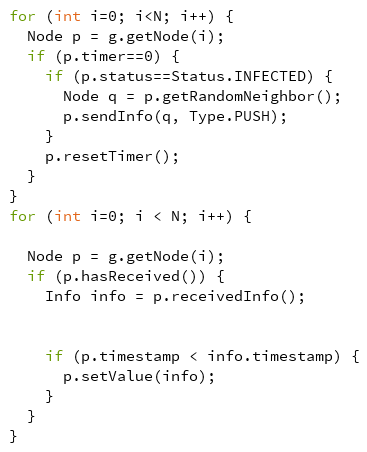
\includegraphics[width=\linewidth,height=8cm]{push-code.png}
      \caption{Push}\label{fig:push_code}
    \end{subfigure}\hfill
    \begin{subfigure}{0.32\textwidth}
      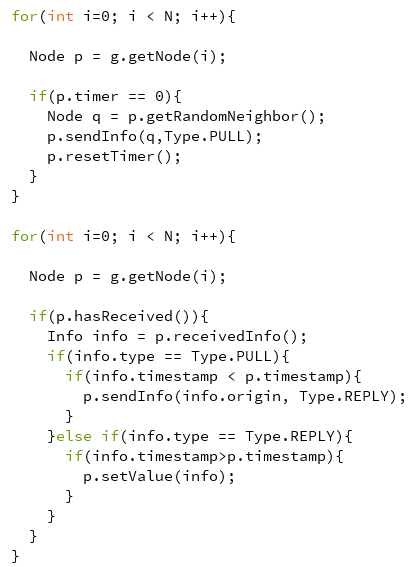
\includegraphics[width=\linewidth, height=8cm]{pull-code.png}
      \caption{Pull}\label{fig:pull_code}
    \end{subfigure}\hfill
    \begin{subfigure}{0.32\textwidth}
      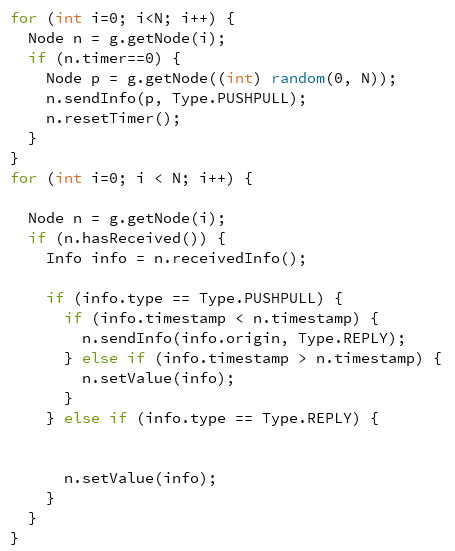
\includegraphics[width=\linewidth, height=8cm]{pushpull-code.png}
      \caption{Pushpull}\label{fig:pushpull_code}
    \end{subfigure}
    \caption{Epidemie semplici}
    \label{fig:simple_epidemics}
    \end{figure}
Il modello SI, chiamato anche anti-entropy o delle epidemie semplici, è il primo protocollo studiato nel centro di ricerca di Xerox. Come già detto, un nodo potrà trovarsi nello stato \textit{susceptible} o \textit{infected}. L'invio periodico di informazioni è scandito da un timer proprio del nodo, impostato inizialmente al valore $\Delta$. Quando il timer scende a zero, il nodo invia il messaggio secondo lo stile scelto ed imposta nuovamente il timer. È interessante notare ogni nodo esegue queste operazioni una sola volta per round.

Nel documento originale vengono esposti e studiati tre stili per il modello SI, che cambiano il modo in cui i componenti della rete comunicano e risolvono le differenze. 

Si utilizzerà la seguente notazione: $n$ indica il numero totale dei nodi presenti sulla rete ($|P|$), mentre i valori $s$ e $i$ indicano rispettivamente il rapporto $|S|/n$ e $|I|/n$. Chiaramente $s + i = 1$.
\subsubsection{Push}
Il primo stile è detto stile push: un nodo infetto sceglierà in modo casuale un vicino a cui inviare informazioni. il nodo destinazione verificherà se le informazioni ricevute sono più aggiornate e, in caso affermativo, cambierà il proprio valore. Un nodo quindi, se infetto, invierà sempre un messaggio ad un altro nodo, indipendentemente dal fatto che il nodo destinazione conosca o meno l'aggiornamento. Si può facilmente intuire che lo stile push è più efficace quando il numero di nodi infetti è basso. In uqesta situazione, infatti, il numero di nodi infetti tenderà a raddoppiare ad ogni round e dopo $O(\log_2 n)$ round il valore $i$ si avvicinerà a $1/2$. Quando invece $i$ supera $1/2$ la situazione cambia: se definiamo $s_t$ il rapporto di nodi suscettibili al roud $t$, possiamo calcolare il numero atteso di nodi suscettibili al round $t + 1$ come:
\begin{equation}
    E(s_{t + 1}) = s_t  \Big(1 - \frac{1}{n}\Big)^{n(1-s_t)}
\end{equation}
Nel dettaglio: un nodo rimane suscettibile se al round $t$ era suscettibile ($s_t$) e non è stato contattato da nessuno dei nodi infetti ($1-1/n$ indica la probabilità che un nodo non contatti il nodo suscettibile, ripetuto per il numero di nodi infetti $n(1-s_t)$).

Questo valore può essere approssimato per $n$ molto grandi a $s_t e^{-(1-s_t)}$. Come dimostra Pittel \cite{pittel} il numero di round atteso $T(n)$ per informare tutti i nodi in una rete è
\begin{equation}
    T(n)= \log_2 n + \ln n + O(1) = O(\log n)
\end{equation}

dove $\log_2 n$ deriva dalla prima fase, $\ln n$ da quella finale, mentre la fase intermedia, molto veloce, dura un numero costante di cicli.
\subsubsection{Pull}
Il secondo stile analizzato è lo stile pull: i nodi chiedono informazioni ad altri nodi, inviando il proprio timestamp. Se questi ultimi possiedono un aggiornamento più recente, invieranno un messaggio in risposta che verrà utilizzato dal nodo iniziale per cambiare il proprio valore.

A differenza dello stile push, quest'ultimo risulta poco efficace quando i nodi infetti sono pochi. Il numero atteso di nodi non ancora infeti dopo $t+1$ round può essere espresso come:
\begin{equation}
    E(s_{t+1}) = s_t \cdot s_t = s_t^2
\end{equation}
in quanto un nodo rimane non informato se nel round precedente era suscettibile ed ha contattato un nodo a sua volta suscettibile. Può accadere che un nodo infetto dovrà aspettare alcuni round prima di venir contattato, rendendo questi round inutili per lo scopo dell'algoritmo. Nonostante ciò, con alta probabilità dopo $O(log n)$ round metà dei nodi sarà infetta. La fase finale invece è molto più rapida in quanto, aumentando il numero di nodi infetti, aumenta la probabilità per un nodo suscettibile di contattare un nodo infetto.
\subsubsection{Push-Pull}
La soluzione migliore proposta si basa su una combinazione dei due stili precedenti. Lo stile push-pull lavora nel modo seguente: all’azzeramento del timer, un nodo invia un messaggio ad un altro nodo scelto tra i vicini in modo casuale, il quale controllerà il timestamp ed a seconda del risultato invierà una risposta oppure aggiornerà il proprio valore. E’ più rapido in quanto sfrutta i punti di forza dei protocolli push e pull (nella fase iniziale sfrutterà il push, nella parte finale il pull). Karp \cite{karp} ha dimostrato che il numero atteso di round per infettare tutti i nodi è $O(\log\log n)$.

Riassumendo, il modello SI è efficace in quanto permette di distribuire su tutta la rete un aggiornamento, in quanto un nodo infetto continuerà (idealmente per sempre) ad inviare o ricevere messaggi. Nonostante ciò questo può rivelarsi un peso non indifferente per la rete in quanto questo modello prevede l’invio del database completo all’interno del messaggio e non il singolo aggiornamento. Se gli aggiornamenti in una rete sono rari, la maggior parte dei messaggi diventa inutile, perché i nodi continueranno a contattarne altri che già sono a conoscenza  dell’aggiornamento. 
\subsection{Epidemie complesse}

\begin{figure}[!htb]
    \begin{subfigure}{0.40\textwidth}
      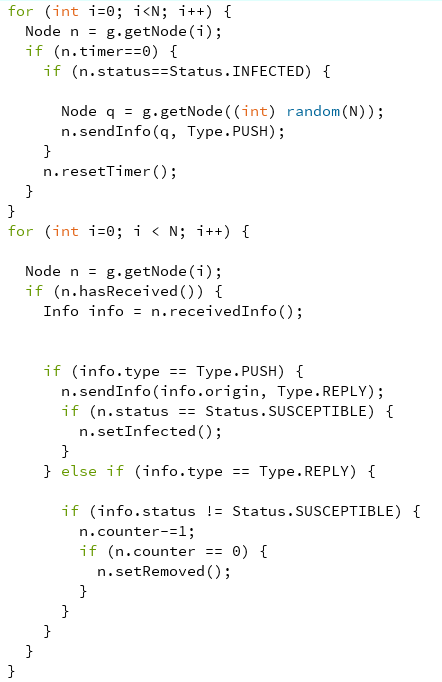
\includegraphics[width=\linewidth,height=10cm]{feedback-counter-code.png}
      \caption{Feedback Counter}\label{fig:feedback_counter_code}
    \end{subfigure}\hfill
    \begin{subfigure}{0.40\textwidth}
      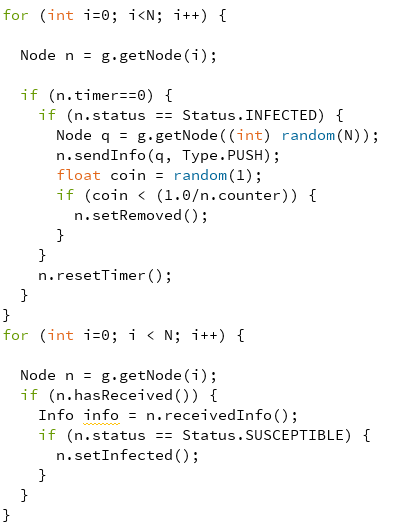
\includegraphics[width=\linewidth, height=10cm]{blind-coin-code.png}
      \caption{Blind Coin}\label{fig:blind_coin_code}
    \end{subfigure}\hfill
    \caption{Epidemie complesse}
    \label{fig:simple_epidemics}
    \end{figure}
Il modello SIR viene introdotto per risolvere il problema della non terminazione del modello precedente e per aumentare l’efficienza. I nodi potranno assumere lo stato rimosso, ovvero nodi che conoscono l’aggiornamento ma non lo distribuiscono più.
Come per le epidemie semplici, inizialmente i nodi sono tutti suscettibili: quando uno di questi viene a conoscenza di un aggiornamento, diventa infetto ed incomincia ad inviare messaggi agli altri nodi. Eventualmente questi nodi potranno “perdere” interesse nel distribuire il proprio aggiornamento, cambiando così il suo stato in rimosso.
Quando nella rete non ci sarà più nessun nodo infetto, l’algoritmo termina.
Il passaggio dallo stato infetto allo stato rimosso può essere influenzato dai seguenti fattori:

\begin{itemize}
    \item \textbf{Come} (How):
    \begin{itemize}
        \item \textbf{counter}: un nodo passerà allo stato rimosso dopo $k$ contatti
        \item \textbf{coin}: un nodo passerà allo stato rimosso con probabilità $1/k$

    \end{itemize}
    \item \textbf{Quando} (When)
    \begin{itemize}
        \item \textbf{feedback}: la valutazione avverrà quando un nodo contatta un altro nodo che era già a conoscenza dell’aggiornamento
        \item \textbf{blind}: la valutazione avverrà ad ogni round
    \end{itemize}
\end{itemize}

Si ottengono così quattro possibili combinazioni: \textit{
feedback/counter, blind/coin, feedback/coin, blind/counter}.
Verranno analizzati \textit{feedback/counter} e \textit{blind/coin} utilizzando lo stile push, ma le considerazioni potranno essere applicate allo stesso modo anche per gli altri algoritmi.

Per confrontare i diversi protocolli che si basano sul modello SIR si utilizzano i seguenti criteri:
\begin{itemize}
    \item \textbf{Residuo}: indica il numero di nodi ancora suscettibili al termine dell’algoritmo (viene indicato con $s^*$). Non è garantito infatti, come invece accade nel modello SI, che tutti i nodi verranno a conoscenza dell’aggiornamento. Può verificarsi una situazione in cui tutti i nodi si trovano nello stato suscettibile oppure rimosso, senza quindi aver ottenuto consistenza in tutta la rete.
    \item \textbf{Traffico}: indica il numero di messaggi inviati. Spesso si utilizza il traffico medio, definito come
    \begin{equation}
        m = \frac{\textrm{traffico totale}}{\textrm{numero di nodi}}        
    \end{equation}
    \item \textbf{Ritardo}: può essere espresso come ritardo medio $t_{avg}$, ovvero la differenza tra il momento dell'infezione iniziale e l'arrivo di un aggiornamento, mediato sul numero di nodi, oppure come ritardo totale $t_{max}$, cioè il tempo necessario affinché l'ultimo nodo riceva l'aggiornamento.
\end{itemize}  
Definiamo, come per il modello SI, $s$, $i$ e $r$ come la il rapporto di nodi suscettibili, infetti e rimossi rispetto al numero di nodi, in modo tale che $s + i + r = 1$.

L’andamento dei seguenti algoritmi può essere modellato attraverso l’utilizzo delle seguenti equazioni differenziali \cite{hethcote}:
\begin{equation}
    \begin{split}
        \frac{ds}{dt} & = - \beta is \\
    \frac{di}{dt} & = \beta is - \gamma i \\
    \frac{dr}{dt} & = \gamma i
    \end{split}
\end{equation}

dove $\beta$ rappresenta il tasso di contagio mentre $\gamma$, chiamato in epidemiologia tasso di recupero, è un valore che dipende da $k$ e dal numero di nodi ancora suscettibili, più precisamente
\begin{equation}
    \gamma = \frac{1}{k}(1-s)
\end{equation}

Possiamo utilizzare le prime due per risolvere il sistema di equazioni differenziali partendo dal loro rapporto e supponendo beta uguale a 1:
\begin{equation}
    \begin{split}
        \frac{di}{ds}   & =  \frac{si - \frac{1}{k} (1-s) i}{-si} \\
        & = \frac{\frac{\cancel{i} (ks - 1 + s)}{k}}{- \cancel{i}s} \\
        & = \frac{1-ks-s}{ks} \\
        & = \frac{1}{ks} - 1 - \frac{1}{k} \\
        & = \frac{1}{ks} - \frac{1+k}{k} 
    \end{split}
\end{equation}
integrando si ottiene
\begin{equation}
    s(i) = \frac{1}{k} \ln s - \frac{1+k}{k} + c
\end{equation}
dove c è costante di integrazione che si può calcolare considerando che inizialmente la funzione è espressa come $i(1-1/n) = 1/n$ che tende a $0$ per $n$ molto grandi

\begin{equation}
    c = \frac{k+1}{k}
\end{equation}
che porta alla seguente soluzione

\begin{equation}
    i(s) = \frac{k+1}{k}(1-s) + \frac{1}{k} \ln s
\end{equation}
Questa equazione può essere utilizzata per calcolare $s^*$ quando $i(s^*) = 0$

\begin{equation}
    s^* = e^{(-k-1)(1-s^*)}
\end{equation}

Il risultato è una funzione implicita su $s^*$, la quale mostra che il residuo diminuisce esponenzialmente all'aumentare di $k$.

È possibile notare inoltre che tutte le varianti dell’algoritmo condividono la stessa relazione tra traffico e residuo. Considerando ogni messaggio inviato ha probabilità pari a 1/n di contattare un nodo specifico, la probabilità di rimanere suscettibile dopo l’invio di m*n messaggi è pari a:

\begin{equation}
    s(m*n) = \Big(1-\frac{1}{n}\Big)^{nm}
\end{equation}

che con $n$ grandi può essere approssimato come $s = e^{-m}$.
Come si può notare dalla tabella 1, il ritardo è l’unico parametro che distingue le varianti: osservando i dati si può notare che feedback/counter offre ritardo inferiore a parità di $k$.




\subsection{Dettagli implementativi}

Nelle pagine precedenti sono stati descritti i protocolli basati sui modelli SI e SIR utilizzati per la distribuzione di informazioni, senza parlare di come questi possano essere utilizzati in casi reali. Innanzitutto anti-entropy e rumor-mongering possono essere utilizzati in contemporanea sulla medesima rete: si suppone infatti che un protocollo basato sul modello SIR può eventualmente terminare senza che si sia ottenuta consistenza su tutta la rete. Per evitare che ciò accada, è possibile eseguire un algoritmo anti-entropy meno frequentemente.


\subsubsection{Valori multipli}

È molto probabile che i protocolli debbano lavorare con più che singoli valori, e quindi la comparazione può diventare molto onerosa. Molto spesso infatti, lavorando con database per esempio, il confronto diventa quasi completamente inutile perché gran parte dei dati sono simili. È possibile risolvere in parte questo problema utilizzando dei checksum calcolati a partire dalla copia del database contenuta nel nodo, ricalcolando ogni volta che quest’ultimo viene aggiornato. Il primo scambio tra nodi avviene attraverso il confronto dei relativi checksum, eseguendo il confronto completo dei database solo se si trovano in disaccordo. Purtroppo la computazione dei checksum tende ad essere molto spesso diversa se l’aggiornamento ai nodi arriva in momenti tanto diversi, quindi la rete tenderà comunque a dover confrontare i dati completi. Una soluzione più complessa prevede di definire un intervallo di tempo che sia sufficiente per far ricevere l’aggiornamento a tutti i nodi. Ogni nodo contiene una lista con gli aggiornamenti più recenti, all’interno di questo spazio di tempo, che viene scambiata ed utilizzata per aggiornare checksum e database. Solo nel caso di un ulteriore disaccordo, viene eseguito il confronto con l’intero database. È importante notare che la scelta dell’intervallo di tempo è cruciale per il funzionamento: se viene fatta in maniera sbagliata, i checksum tenderanno a differenziarsi, aumentando il traffico rendendolo superiore al traffico generato dai protocolli anti-entropy senza checksum.

Un' ultima soluzione, che non prevede la scelta a priori di un intervallo di tempo, prevede la memorizzazione di un indice inverso del database basato sul timestamp. I nodi si scambiano gli aggiornamenti in ordine inverso di timestamp, ricalcolando i checksum fino ad ottenere un consistenza di questi ultimi. Non è comunque ottimale a causa del costo di mantenimento dell’indice inverso in ogni nodo.

\subsubsection{Traffico generato}
Un problema non trascurabile in casi reali è sicuramente il traffico che una rete può supportare. Questi protocolli prevedono che ad ogni round vengano inviati più messaggi contemporaneamente, rischiando quindi di sovraccaricare la rete. Demer aveva definito questo come connection limit, spiegando che definire un limite è necessario sia in caso di puh che di pull. Questa condizione porta però ad un significativo peggioramento dei protocolli che utilizzano lo stile pull, mentre push diventa migliore. Il protocollo Scuttlebutt \cite{flowgossip} definisce alcuni rimedi a questa limitazione, specificando un metodo per determinare in modo dinamico il tasso massimo di traffico che un nodo può generare senza dover creare un sistema di backlog per gli aggiornamenti. 

\subsubsection{Gestione dei fallimenti}
Implementando i protocolli di gossip in contesti reali comporta il rischio di possibili fallimenti per fattori esterni. Per fortuna, la perdita di messaggi non aggrava sull’esecuzione se non rallentando il raggiungimento della consistenza (alcuni round diventano inutili). Se alcuni nodi smettono di “funzionare”, gli scambi con questi diventano inutili e i protocolli rallentano la loro esecuzione. È comunque auspicabile mantenere lo stato attivo degli endpoint in modo da evitare questi inconvenienti.

\section{Altri utilizzi dei protocolli epidemici}

Negli scritti di Demers \cite{demers}, si supponeva che la rete fosse statica, ovvero il numero di nodi rimaneva fisso nel tempo. Inoltre ogni nodo aveva una visione totale, e quindi il grafo rappresentativo era completo. Infine il numero di macchine collegate era relativamente basso.
Oggigiorno le reti sono molto più grandi, non sono completamente connesse e la lista di nodi direttamente connessi tra loro può variare per continue connessioni-disconnessioni. Questo sicuramente porta grandi vantaggi, come una maggior scalabilità. I protocolli epidemici possono essere adattati a questi grandi cambiamenti ed utilizzati per altri scopi, oltre alla distribuzione di informazioni. Esistono implementazioni dei protocolli epidemici per mantenere informazioni sullo stato di una rete peer-to-peer \cite{newscast}, per rilevare errori e guasti \cite{swim}, per implementare garbage collection \cite{garbage_collection}, per calcolare informazioni di aggregazione \cite{aggregation}, …
\subsection{Notazione}

Si può definire un algoritmo di gossip generico, che si basa sulle implementazioni precedenti e descrive i vari momenti che devono essere tenuti in considerazione:
\begin{itemize}
    \item \textbf{inizializzazione}: un nodo viene definito con il suo stato iniziale. Viene impostato il timer
    \item \textbf{allo scadere del timer}: il nodo sceglie un vicino, prepara il messaggio, lo invia al nodo scelto e reimposta il timer
    \item \textbf{al ricevimento di un messaggio di richiesta}: il nodo prepara la risposta e la invia. Il nodo legge la richiesta e la elabora
    \item \textbf{al ricevimento di un messaggio di risposta}: il nodo elabora la risposta.
\end{itemize}

Da queste situazioni si può notare come i metodi di elaborazione ed invio non sono stati implementati, ma questa operazione verrà fatta in seguito. 

\section{Peer sampling}

Per la gestione di reti dinamiche e di grandi dimensioni, il mantenimento di una lista contenente tutti i nodi è oneroso e per nulla efficiente. A causa della possibilità di fallimenti o di nuovi nodi, questa lista deve essere aggiornata frequentemente, per poi essere diffusa a tutti. 

Per risolvere questo problema si utilizza un sottoinsieme della lista completa, scelta per ogni nodo in maniera casuale. Il mantenimento di questo sottoinsieme è sicuramente più gestibile. 
Il metodo che si occupa di questo compito è chiamato \texttt{getPeer()}.
Di seguito la spiegazione di Newscast \cite{newscast}, un protocollo di membership management (un altro modo per chiamare il peer sampling).

\subsection{Definizione del problema}
Il protocollo Newscast funziona nel modo seguente: ad ogni round un nodo sceglie un vicino casuale tra la sua vista parziale di $c$ elementi. Successivamente, stabilita la connessione, i nodi si inviano reciprocamente una la loro lista più il proprio indirizzo con il timestamp aggiornato. Infine stilano una lista dei $c$ collegamenti più recenti, eliminando i restanti.
L’algoritmo generico viene completato nel seguente modo:
\begin{itemize}
    \item \texttt{selectNeighbor()}: sceglie un nodo dalla vista parziale
    \item \texttt{prepareRequest()} e \texttt{prepareReply()}: ritorna la vista parziale completa del nodo più il proprio indirizzo con il timestamp o un identificatore aggiornato
    \item \texttt{mergeRequest()} e \texttt{mergeReply()}: ritorna i più recenti descrittori, scelti tra la propria vista e quella inviata dall’altro nodo
\end{itemize}
Per entrare nel sistema, un nodo deve conoscere l'indirizzo di almeno un nodo già presente nella rete. Successivamente il nodo invia la propria vista parziale, ed aggiunge alla sua vista il nuovo nodo, con un identificatore aggiornato [Mont]. Utilizzando questo algoritmo, le viste parziali continueranno a cambiare, aggiornando gli identificatori di conseguenza. Se un nodo deve lasciare la rete, non serve che svolga azioni particolari. Il suo identificatore non verrà più aggiornato ed eventualmente diventerà vecchio a tal punto da non essere più salvato nelle viste dei nodi.

Dall'analisi fatta in \cite{membership}, il protocollo possiede le seguenti proprietà:
\begin{itemize}
    \item \textbf{self-organizing}: l'algoritmo funziona senza necessità di controllo manuale anche se i nodi in modo casuale entrano oppure lasciano la rete
    \item \textbf{effective}: l'informazione è distribuita in modo veloce e prevedibile
    \item \textbf{scalable}: il protocollo non da problemi anche se il numero di nodi è elevato
    \item \textbf{robust}: il sistema tollera danni anche gravi
\end{itemize} 

\section{Failure detection}
La rilevazione di errori in sistemi distribuiti è un problema complesso \cite{failure_detection} principalmente perché molto spesso un processo può sembrare problematico anche se in realtà è semplicemente lento oppure la connessione è limitata. È necessario verificare con accuratezza che un nodo sia “guasto”, in modo da limitare il più possibile i falsi positivi mantenendo una conoscenza parziale dei nodi il più aggiornata possibile. 
\subsection{Definizione del problema}
Il protocollo SWIM \cite{swim} offre un sistema di failure detection e, utilizzando il principio del gossip, un modo scalabile ed efficiente per distribuire le informazioni ricevute, mantenendo così aggiornata la lista dei membri che ogni nodo possiede. Si può dire quindi che combina sia il membership management e la failure detection.

Il problema della scalabilità delle precedenti soluzioni è dovuto principalmente all’utilizzo della tecnica di heartbeating: un membro Mi è dichiarato guasto da un altro membro Mj quando non riceve messaggi “heartbeat” (messaggi con counter incrementale) per un determinato numero di periodi consecutivi \cite{swim}.
\subsection{Algoritmo}
L’algoritmo è realizzato in modo da dividere le componenti di failure detection e di membership update, senza utilizzare il metodo heartbeat \cite{swim}:
\begin{itemize}
    \item \textbf{failure detection}: componente che rileva i guasti
    \item \textbf{dissemination}: componente che invia informazioni riguardo i membri che entrano o lasciano la rete
\end{itemize}

\textbf{SWIM Failure Detector} Utilizza due parametri: $T$ indica il periodo del protocollo, mentre $k$ indica il numero di nodi appartenenti al gruppo che si occupa di contattare un nodo che non ha inviato risposte. Ad ogni round (di lunghezza $T$), un nodo $M_i$ sceglie un altro nodo $M_j$ dalla sua lista di vicini e invia un messaggio \textit{ping} e aspetta la risposta \textit{ack}. Se questa non arriva dopo un determinato periodo, inferiore a $T$, $M_i$ contatta i $k$ nodi scelti all’avvio del protocollo e chiede loro, attraverso un messaggio \textit{ping-req}, di contattare il nodo $M_j$. Se nessuno di questi nodi riceve risposta ed invia la conferma della salute del nodo $M_j$, questo viene dichiarato guasto nella lista di $M_i$, che si occuperà di distribuire la scoperta a tutta la rete.
\textbf{Dissemination component} Se un nodo imposta un nodo come guasto, inizia a distribuire questa informazione a tutta la rete. La versione base del protocollo SWIM utilizza un sistema multicast, mentre una versione più robusta sfrutta il principio della diffusione delle epidemie, quindi i protocolli epidemici.
\subsection{Riduzione dei fasi positivi}
La versione base del protocollo SWIM rischia di aumentare il numero di nodi considerati guasti nel caso di perdita di pacchetti oppure per una temporanea disattivazione del nodo in questione. Per evitare questo problema viene introdotto protocollo  chiamato Suspicion protocol \cite{swim}: quando un nodo Mi non riceve informazioni da un nodo Mj, ne dai nodi che lo aiutano a contattarlo, imposta il nodo $M_j$ come Sospetto. Se un altro nodo riceve questa informazione, marca nella sua lista il nodo come sospetto.

Se un nodo riesce a contattare un nodo sospetto, comincia ad inviare un messaggio $Alive(M_j)$, il quale sovrascrive il sospetto di guasto. Quando un nodo rimane sospetto per un certo periodo di tempo, senza avere ulteriori informazioni, viene marcato come guasto in modo definitivo. Oltre allo stato di \textit{Suspect/Alive/Confirm}(guasto), viene associato anche un contatore, generato in modo da gestire la successione di messaggi e la loro eventuale sovrascrittura all’interno della lista.

\section{Aggregazione}
I protocolli epidemici possono essere utilizzati anche per calcolare una determinata proprietà del sistema. Permettono quindi di conoscere informazioni che altrimenti sarebbero note solo avendo una conoscenza globale della rete. Possono essere utilizzati per calcolare il numero di nodi collegati, la media dei loro valori, il massimo o il minimo, lo spazio libero su disco, ... \cite{montresor}.

\subsection{Media di valori}
Si suppone che ogni nodo possiede un singolo valore. L'obiettivo è calcolare la media di questi valori utilizzando i protocolli epidemici. Le funzioni generiche di un protocollo di gossip vengono definite nel modo seguente
\begin{itemize}
    \item \texttt{prepareRequest()} e \texttt{prepareReply()}: ritornano il valore contenuto nel nodo
    \item \texttt{mergeRequest()} e \texttt{mergeReply()}: ritornano una media locale tra il valore del nodo ed il valore ricevuto
\end{itemize}
Alla fine di uno scambio di informazioni, la somma totale dei valori dei nodi della rete rimane invariata, quindi l'algoritmo è corretto, ma allo stesso tempo diminuisce la varianza. Quando la varianza tra i valori tende a zero, il valore contenuto nei nodi sarà lo stesso, e sarà uguale alla media dei valori iniziali.

Questo algoritmo da problemi nel caso di scambi di informazioni contemporanei. Se infatti un nodo $r$ contatta un nodo $p$, il quale ha già instaurato una connessione con un altro nodo $q$ senza però ricevere ancora risposta, la somma dei valori alla fine dello scambio non corrisponde a quella iniziale. Sia infatti $e_p$, $e_q$ e $e_r$ i valori precedenti lo scambio, allora dopo lo scambio $q$ conterrà $\frac{e_p+e_q}{2}$, $r$ conterrà $\frac{e_p + e_r}{2}$, mentre $p$ conterrà $\Big(\frac{e_p+e_r}{2} + e_q\Big) / 2$ la cui somma totale è $\frac{5e_p + 4 e_q + 3e_r}{4}$ chiaramente diversa da $e_p+e_q+e_r$.

Si può risolvere il problema in due modi: rifiutare di comunicare con $r$ prima che la risposta sia arrivata, oppure cambiare l'implementazione delle funzioni nel seguente modo:
\begin{itemize}
    \item \texttt{prepareRequest()}: ritorna il vlaore del nodo
    \item \texttt{prepareReply()}: crea una nuova variabile $d=value - (value + req)/2$ dove $req$ è il valore ricevuto dal nodo
    \item \texttt{mergeRequest()}: ritorna il valore sotrraendo $d$
    \item \texttt{mergeReply()}: ritorna il valore sommando $d$
\end{itemize}


\subsection{Altre funzioni di aggregazione}
Oltre alla media si possono calcolare altri valori interessanti della rete
\begin{itemize}
    \item calcolo del minimo o del massimo: basta utilizzare le funzioni \texttt{prepareRequest()} e \texttt{prepareReply()} per ritornare il valore, mentre \texttt{mergeRequest()} e \texttt{mergeReply()} calcolano il massimo o il minimo tra i due valori
    \item calcolare il numero di nodi in una rete: si parte con un nodo con valore inizializzato a $1$, e gli altri  a $0$. Dopo aver eseguito l'algoritmo per un certo numero di round il valore contenuto in ciascun nodo sarà pari a $1/n$, quindi è basilare calcolare $n$
    \item calcolare il totale: dopo aver calcolato la media, basta moltiplicarla per il numero di nodi nella rete 
\end{itemize}
\subsection{Dettagli implementativi}
I protocolli di aggregazione presentati non tengono pero' conto della dinamicita' delle reti. Per ottenere valori aggiornati e reali questi protocolli devono essere periodicamente riavviati: i nodi salvano il valore corrente e lo utilizzano per l'avvio successivo, eseguendo il protocollo per un determinato numero di round. La singola esecuzione del protocollo e' detta epoca.
Inoltre in sistemi con un numero di nodi molto elevati, l'esecuzione del protocollo in modo sincronizzato non e' fattibile. Il passaggio da un'epoca all'altra avviene nel momento in cui il nodo scopre un nuovo identificatore di epoca.
\section{Conclusioni}
Grazie alla loro efficienza e robustezza quando utilizzati in sistemi distribuiti, i protocolli epidemici sono sempre piu' utilizzati ed approfonditi. Come spiegato nelle sezioni precedenti, il loro utilizzo non si limita solamente alla diffusione di informazioni, ma anche ad altre apllicazioni quali la gestione della rete o l'acquisizione di dati globali difficilmente ottenibili in altri modi. Anche se inizialmente sono stati utilizzati in reti limitate e statiche, sono stati poi adattati ed ottimizzati anche per reti di grandi dimensioni che possono cambiare la loro topologia durante l'esecuzione dell'algoritmo stesso.








      \newpage
\chapter{Relazione tirocinio}
\label{cha:conclusioni}


In questo capitolo viene esposto un resoconto del tirocinio avvenuto tra i mesi di aprile e maggio 2019 presso il Liceo Galileo Galilei (Trento), il liceo Leonardo Da Vinci (Trento), l’istituto tecnico tecnologico Buonarroti-Pozzo (Trento) e il liceo Scientifico presso il collegio Arcivescovile Celestino Endrici (Trento). L’attività è stata strutturata in due parti: una parte teorica di lezione interattiva e una parte laboratoriale in cui i ragazzi svolgevano degli esercizi. Lo scopo del tirocinio è stato quello di proporre un modo diverso di visualizzare ed utilizzare l’informatica presso gli istituti superiori, seguendo i principi del modello Computational STEAM (\autoref{chap:steam}). L’argomento trattato, i protocolli epidemici (\autoref{chap:epidemic}), è stato scelto perché adatto a far comprendere come modelli e algoritmi studiati in altri campi (la biologia e la matematica) possano essere adattati ed utilizzati con efficacia in ambito informatico (nello specifico la comunicazione in sistemi distribuiti).
\section{Contesto}
Essendo tre studenti abbiamo organizzato questa esperienza di tironcio nel seguente modo: ognuno ha portato un argomento diverso, ma con le stesse modalità di presentazione (seguendo i principi di Computatonal STEAM) in tre classi per un totale di 9 classi.
Abbiamo presentato il corso tra aprile e maggio presso i seguenti istituti superiori: liceo Scientifico Galileo Galilei di Trento, liceo Scientifico Leonardo Da Vinci di Trento, liceo Scientifico collegio Arcivescovile Celestino Endrici e istituto tecnico e tecnologico Buonarroti-Pozzo. Abbiamo scelto questo periodo in quanto più adatto sia per i ragazzi che per gli insegnanti ordinari. Ci siamo concentrati sul liceo scientifico, in quanto il percorso di studi Computational STEAM è indirizzato a questa tipologia di scuola, ma abbiamo deciso di provare a portare l’esperienza anche in un istituto tecnico, per cercare di capire quali possono essere le differenze riguardo la preparazione dei ragazzi, in modo da adattare le lezioni al meglio. 

Il nostro obiettivo consisteva nel proporre dei corsi durante le ore di informatica, trattando tematiche che si interfacciassero ad altre materie studiate dai ragazzi. Dai dati raccolti abbiamo notato che questa metodologia, proposta sia all'interno della riforma Gelmini del 2010 \cite{riforma} sia tra i principi fondanti di Computational STEAM, spesso non è applicata: alcuni ragazzi conoscevano le potenzialità dell'informatica come scienza computazionale, mentre per altri è stata una novità. 

Le classi a cui sono rivolti sono terze, quarte e quinte, perché gli argomenti trattati risultano più adatti a studenti con conoscenze che vengono fornite a partire dal terzo anno in poi. La scelta delle classi è stata fatta dagli insegnanti di informatica, a cui sono stati proposti i moduli.


\section{Organizzazione del corso}
Abbiamo strutturato le lezioni nel seguente modo: un’ora per l’introduzione, e le restanti 6 ore per il contenuto del corso in sè. La lezione introduttiva e l’ultima sono state utilizzate anche per compilare un questionario introduttivo ed un conclusivo (entrambi anonimi), i cui risultati sono utilizzati come supporto alla stesura di questo capitolo. È stata utilizzata l’applicazione Moduli Google. Abbiamo raccolto le risposte di 164 ragazzi per il questionario iniziale, 161 per quello finale. Questi sono i dati aggregati per tutte le classi. Utilizziamo i dati aggregati per la parte  di contesto, mentre per la parte "tecnica" li suddividiamo in base al corso frequentato (alcune domande sono specifiche del modulo, come quelle riguardante il feedback riscontrato, il quale può variare in base a chi ha presentato il corso). 

Per quanto riguarda il corso sui protocolli epidemici, è stato distribuito in singole ore (da 50 minuti, come previsto per gli istituti superiori)ad eccezione dell'istituto tenico e tecnologico Buonarroti, in cui si è svolto in blocchi di 3 ore e un esperimento al liceo Da Vinci con una lezione di due ore, in cui è intervenuta la professoressa di scienze per portare alcune riflessioni riguardo la diffusione delle epidemie, spiegando quali sono state le pandemie piu' importanti della storia e come si sono diffuse. Abbiamo notato che svolgere le lezioni in blocchi di almeno due ore permette di approfondire maggiormente le tematiche affrontate, lasciando spazio ai ragazzi di completare gli esercizi. Con lezioni della durata di un'ora talvolta sgli studenti sono costretti a lasciare incompleti gli esercizi, per poi riprenderli l'ora successiva. 

\begin{figure}[!ht]
    \begin{subfigure}{.5\textwidth}
        \centering
        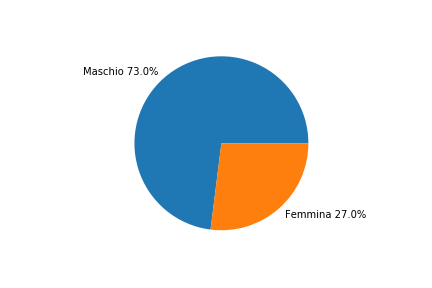
\includegraphics[width=\textwidth]{genere.png}
        \caption{Genere}
        \label{fig:genere}
    \end{subfigure}\hfill
    \begin{subfigure}{.5\textwidth}
        \centering
        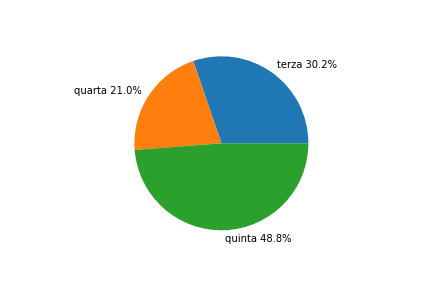
\includegraphics[width=\textwidth]{classi.png}
        \caption{Classi}
        \label{fig:classi}
    \end{subfigure}
    \caption{Caratteristiche del campione} 
\end{figure}
\subsection{Analisi del campione}
Le classi sono prevalente composte da maschi, il che non è affatto sorprendente osservando la composizione nei corsi di studio di informatica ed ingegneria. I ragazzi hanno notato questa differenza numerica, motivandola principalmente con questa affermazione: “l'informatica è preferita dai ragazzi”. Nonostante ciò, la figura dell’informatico è stata descritta in modo abbastanza lontano dai frequenti stereotipi: secondo i dati raccolti molti pensano che un informatico debba essere creativo e debba avere capacità nel lavorare in gruppo.

\begin{figure}[!ht]
    \centering
    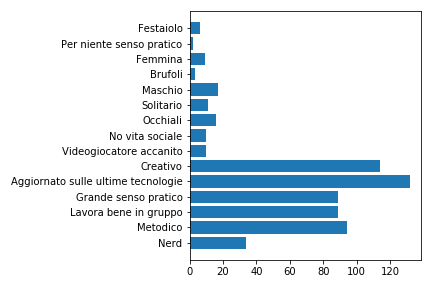
\includegraphics[height=8cm]{computer_scientist.png}
    \caption{Quali sono i requisiti per essere un perfetto informatico?}
    \label{fig:computer_scientist}
\end{figure}

Ai ragazzi è stato chiesto quanto apprezzano la materia in sè e come questa venga insegnata attualmente: i risultati presentano un giusto equilibrio, con alcuni studenti che la preferiscono ed altri che la disprezzano o non ne trovano l'utilità. Attraverso queste lezioni abbiamo cercato di trasmettere l'importanza dell'informatica, dimostrando che puo' rivelarsi divertente e interessante, senza ovviamente ricadere nella banalità.

\section{Contenuto e metodo esecutivo} 
Il contenuto del corso è stato esposto utilizzando delle slide per la parte di lezione teorica, mentre per la parte applicativa è stata fornita una cartella condivisa con gli esercizi da svolgere e le loro spiegazioni nel dettaglio (\href{http://www.tinyurl.com/protocolli-epidemici}{http://www.tinyurl.com/protocolli-epidemici}). Questo spazio è stato aggiornato durante il corso, aggiungendo nuovo materiale e correggendo errori e sviste notate dai ragazzi. All'interno si possono trovare, oltre alle istruzioni per una corretta installazione di Processing, un documento con la descrizione della libreria e degli esercizi da svolgere, il codice di partenza per eseguire gli esercizi, i lucidi proiettati durante le lezioni, il file compilato della libreria e una serie di link utili, per coloro che vogliono approfondire gli argomenti trattati (tra cui Processing e la diffusione delle epidemie) attraverso tutorial, articoli e libri. 

La parte teorica è stata presentata come lezione interattiva, dando spazio agli studenti di porci delle domande e di rispondere a quesiti da noi proposti. Ad eccezione della prima ora di lezione, tutte le altre hanno avuto una componente pratica, in modo tale che i ragazzi potessero applicare quanto imparato. La difficoltà degli esercizi è via via crescente, sia per la complessità degli algoritmi proposti, sia per un minore aiuto fornito in determinate situazioni (in alcuni casi è stato fornito solamente lo pseudocodice). 

Tra i vari argomenti possibili ho scelto di sviluppare il corso sui protocolli epidemici (vedi \autoref{chap:epidemic}) per diversi motivi: in primo luogo, l’argomento si basa su semplici regole che vengono utilizzate più volte in diversi contesti. I protocolli di gossip possono però essere studiati maggiormente e lasciano spazio anche ad un approfondimento autonomo. Inoltre sono sono un argomento interdisciplinare: vengono utilizzati in reti distribuite per la comunicazione, ma i principi su cui si basano sono studiati in epidemiologia, nell’ambito quindi della diffusione delle epidemie, ma anche dalle scienze sociali, riguardo il fenomeno del gossip. Questa interdisciplinarietà si dimostra adatta all’interno di questa esperienza che vuole portare i principi di Computational STEAM nelle scuole superiori.

Nello specifico ho sviluppato il programma del corso nel seguente modo: nella prima lezione, utile come introduzione, ho presentato l’argomento e la sua natura interdisciplinare, il contesto storico, la definizione del problema, le applicazioni reali e i principi di base.
\begin{figure}[!ht]
    
    \begin{subfigure}{.5\textwidth}
        \centering
        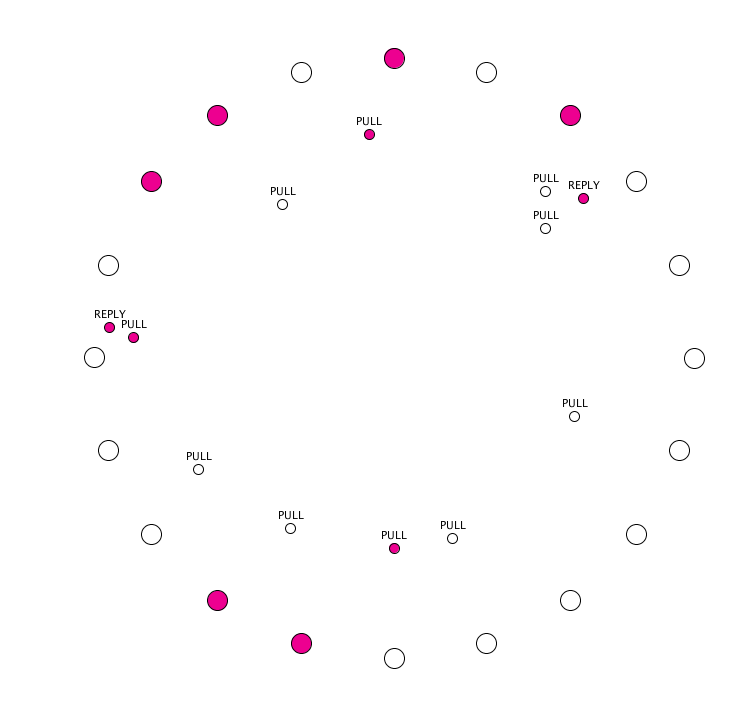
\includegraphics[width=\textwidth]{pull.png}
        \captionsetup{justification=centering}
        \caption{Algoritmo modello SI: pull} 
    \end{subfigure}\hfill
    \begin{subfigure}{.5\textwidth}
        \centering
        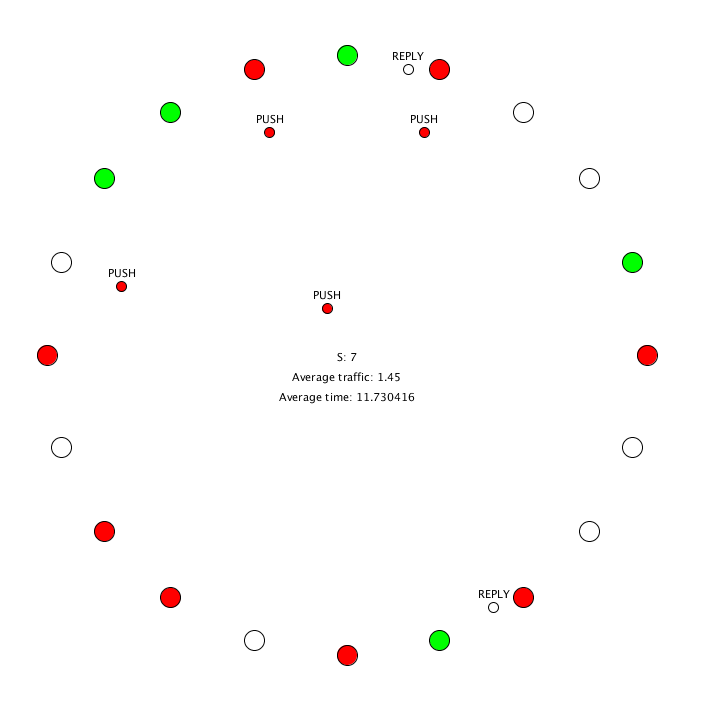
\includegraphics[width=\textwidth]{feedback-counter.png}
        \captionsetup{justification=centering}
        \caption{Algoritmo modello SIR: feedback-counter} 
    \end{subfigure}
    \caption{Esempi di output}
    \label{fig:output}
\end{figure} 

Nelle successive lezioni mi sono concentrato, dopo aver fatto una breve introduzione sui grafi (utile per alcune definizioni), sui due modelli SI e SIR presentando gli algoritmi e stili che li utilizzano, lasciando poi spazio ai ragazzi di implementarli su schermo. Una lezione tipo è stata organizzata nel seguente modo: nella prima parte viene introdotto il modello e viene definito il problema. Poi vengono introdotte le componenti necessarie, i metodi della libreria utili per la risoluzione. Infine viene esposto lo pseudocodice, che suddivide i momenti fondamentali dell'esecuzione degli algoritmi: allo scadere del timer e alla ricezione delle informazioni. Nel tempo restante della lezione i ragazzi cercano di trovare una soluzione al problema, completando gli esercizi (l'output di alcuni esercizi in Figura \ref{fig:output}).

L’ambiente di sviluppo utilizzato è Processing (\href{https://processing.org}{https://processing.org}), libreria grafica di Java e IDE utile per creare simulazioni e metodi di visualizzazione efficace \cite{processing_wikipedia}. La versione utilizzata è la 3.5.3: è stata installata prima dell'inizio del corso sulle macchine dei laboratori con sistema operativo Windows 10.

Ho fornito una libreria (\href{https://github.com/ainter21/epidemic}{https://github.com/ainter21/epidemic}), utile sia per alleggerire il carico di lavoro, sia per nascondere alcune componenti troppo complesse, come la parte di visualizzazione (lo scopo degli esercizi è quello di implementare l’algoritmo, mentre la parte di visualizzazione è solamente un supporto per rendere più chiari i concetti).
Ho fornito la documentazione utile per completare gli esercizi, con la spiegazione dei metodi e degli attributi. Il loro obiettivo è stato quindi utilizzare la libreria fornita (con metodi molto simili a quelli utilizzati nell' pseudocodice), affinché gli algoritmi proposti funzionassero. La lista degli esercizi proposti già completati è scaricabile qui (\href{https://github.com/ainter21/epidemic-protocols}{https://github.com/ainter21/epidemic-protocols}).

Le attività sono state svolte nei laboratori di informatica, in modo tale da poter proiettare i lucidi e permettere ai ragazzi di lavorare in autonomia o a gruppi. L'idea iniziale era di formare dei gruppi di lavoro per poter collaborare e sviluppare abilità di problem solving e lavoro di squadra. Questa soluzione si è rivelata di difficile attuazione in quanto i ragazzi possiedono un account personale non condivisibile e se alcuni studenti rimanevano assenti, si rischiava di non poter accedere al lavoro iniziato la volta precedente. Abbiamo comunque fatto il possibile per invogliarli a lavorare in gruppo.

\subsection{Libreria nel dettaglio}
La libreria è stata scritta in modo tale da nascondere la parte di programmazione ad oggetti non studiata dai ragazzi al liceo scientifico. Le classi principali sono: \texttt{Graph}, \texttt{Node} e \texttt{Info}. La rete è visualizzata attraverso un grafo. Ho associato il valore interno del nodo ad un colore, per rendere l'output visivo piú accattivante.

I ragazzi hanno utilizzato i metodi già implementati nei vari oggetti (specialmente nella classe \texttt{Node}) per eseguire azioni e acquisire informazioni. Il grafo creato è completo, assunzione che durante le lezioni non è stata rilassata per mancanza di tempo.

All'interno della libreria è presente una classe astratta \texttt{Graph}, da cui sono definiti grafi dei rispettivi modelli: \texttt{GraphSI}, \texttt{GraphSIR} e \texttt{GraphAggregation}. Vengono inizializzati come grafi completi, in quanto durante il corso è stata fatta questa assunzione. Ogni grafo ha un metodo utilizzato per aggiornare le sue componenti \texttt{updateGraph()} ed uno per disegnarlo ad ogni frame di esecuzione \texttt{drawGraph()}. 

La seconda classe, \texttt{Node}, oltre al metod per disegnarla \texttt{drawNode()}, è fornita di metodi utili per aggiornare il valore (\texttt{setValue()}, \texttt{setInfected()} e \texttt{setRemoved()}), per resettare il timer interno \texttt{reseTimer()} e per inviare le informazioni \texttt{sendInfo(target, type)}. Quest'ultimo metodo istanzia un ulteriore oggetto, \texttt{Info}, utile per contenere tutti i dati che devono essere poi processati nel momento in cui l'informazione arriva a destinazione (secondo gli algoritmi e i modelli spiegati nel \autoref{chap:epidemic}).

I ragazzi hanno comunque avuto la possibilità di leggere il codice e di modificarlo, compilando la propria versione della libreria.
\section{Analisi dei risultati}

\begin{figure}[ht]
    
    \begin{subfigure}{.5\textwidth}
        \centering
        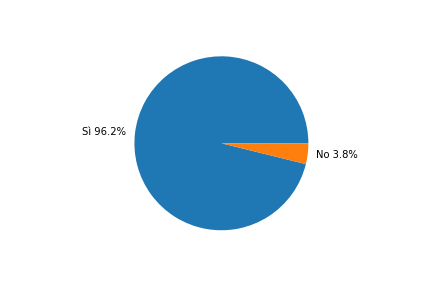
\includegraphics[width=\textwidth]{aspettative.png}
        \captionsetup{justification=centering}
        \caption{Ritieni che siano state \\ soddisfatte le tue aspettative?} 
    \end{subfigure}\hfill
    \begin{subfigure}{.5\textwidth}
        \centering
        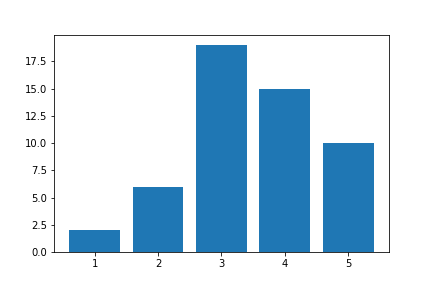
\includegraphics[width=\textwidth]{conoscenze.png}
        \captionsetup{justification=centering}
        \caption{Quanto il corso era adatto  \\ al tuo livello di conoscenze?} 
    \end{subfigure}
    \caption{Risultati}
\end{figure} 

Dopo le sette ore previste, abbiamo chiesto di compilare un questionario di valutazione delle attività svolte.  I dati analizzati in questa sezione non sono i dati aggregati: 60 risposte per il questionario iniziale, e 52 per il questionario finale, ovvero quelle riguardanti il modulo "protocolli epidemici".

I risultati sono positivi, la maggior parte degli studenti dice di essere rimasto soddisfatto. Gli argomenti trattati erano una novità per la maggior parte dei ragazzi, ed alcuni hanno riferito di voler approfondire l'argomento (sia per quanto riguarda l'utilizzo di Processing, sia per i protocolli epidemici, sia per la diffusione delle epidemie). 

Avendo portato il corso sia in un liceo che in un istituto tecnico abbiamo notato alcune differenze, a causa del programma svolto dai ragazzi e dal numero di ore assegnate all'informatica. I ragazzi del liceo, non avendo programmato ad oggetti, si sono trovati in difficoltà nel comprendere alcuni concetti. Conoscevamo già il programma svolto ed il livello di preparazione, ma abbiamo comunque optato per l'utilizzo di Processing e quindi di Java, in quanto avrebbe reso piú accattivante il risultato finale per i ragazzi. Alcuni ragazzi hanno avuto piú difficoltà nel lavorare in gruppo perché, da quanto capito, non è una tecnica molto utilizzata durante l'anno. Inoltre si sono trovati spaesati nel momento in cui abbiamo dato loro autonomia nello svolgere gli esercizi: alcuni hanno avuto difficoltà nel completare gli esercizi. Ai ragazzi è stato suggerito di scrivere su carta, riflettere in gruppo per cercare una possibile soluzione, ma questo consiglio non è stato molto seguito e la maggior parte ha iniziato a scrivere immediatamente codice, con risultati non sempre soddisfacienti. In alcuni casi è stato mostrato dello pseudocodice in modo da dare un punto di partenza: all'istituto tecnico era già stato utilizzato questo metodo, quindi questo materiale è risultato piú utile.

Anche l'utilizzo di una libreria è stata una novità per i ragazzi: hanno sperimentato questa potenzialità dei linguaggi di programmazione consultando la documentazione fornita, cercando di capire quali metodi e attributi fossero adatti alla situazione. Anche se all'inizio si sono trovati un po' spaesati, con il procedere del corso hanno preso dimestichezza con il metodo proposto.

Sarebbe stato anche utile investire alcune ore per introdurre in modo piú approfondito l'ambiente di sviluppo, ma purtroppo il tempo era limitato e questo avrebbe ridotto lo spazio dedicato all'argomento principale del corso. Il codice Processing può essere scritto in diversi linguaggi di programmazione oltre a Java: Python e Javascript. Si potrebbe provare a portare questi corsi utilizzando il linguaggio Python, piú semplice rispetto a Java (è stato scelto Java perché simile al C++, utilizzato durante l'anno dai ragazzi). Python presenta alcuni vantaggi rispetto ad altri linguaggi, specialmente nel contesto degli istituti superiori: come viene fatto notare da Grandell e colleghi in \cite{python_high_school}, questo linguaggio ha una sintassi piú semplice rispetto ai linguaggi normalmente utilizzati, è tipizzato dinamicamente (può essere uno svantaggio, ma riduce la quantità di codice) ed oggigiorno è sempre piú utilizzato anche nel mondo del lavoro. Inoltre le potenzialità di Python emergono anche dal grande numero di moduli che possono essere aggiunti. 

In conclusione si può dire che l'esperienza ha avuto esito positivo leggendo i feedback dei ragazzi ed è stato utile a noi per capire in che modo proporre un argomento esterno al programma scolastico presentandolo con modalità diverse da quelle classiche. è stato utile ai ragazzi per capire come l'informatica possa essere applicata ed utilizzata come materia interdisciplinare e di supporto e come altre materie si possono interfacciare all'informatica ("ho conosciuto delle sue applicazioni molto interessanti ", "Ho cambiato idea sull'applicazione dell'informatica in campi diversi, penso che sia un buon supporto!"). Nel caso venga riproposta un'esperienza simile, è auspicabile che i ragazzi abbiano già un conoscenza di base riguardo la programmazione ad oggetti e l'ambiente di sviluppo Processing in modo da rendere piú comprensibili alcuni concetti e dare piú libertà ai ragazzi nello scrivere il codice (il dover partire da zero a scrivere il codice leggendo la documentazione della libreria è stato uno scoglio troppo grande da superare, quindi gli esercizi sono stati presentati in modo guidato, cone delle parti da completare).

      \newpage
\chapter*{Conclusioni} % senza numerazione
\label{conclusioni}

\addcontentsline{toc}{chapter}{Conclusioni} % da aggiungere comunque all'indice

La proposta di un corso di studi superiori basato sui principi di STEAM e con l'integrazione dell'informatica non solo come materia per tecnici del settore, può essere un grande passo in avanti nella riforma dell'istruzione in Italia. L'informatica negli anni ha assunto sempre più importanza nelle nostre vite grazie al rapido sviluppo tecnologico: è quindi necessario formare dei ragazzi consapevoli delle potenzialità che questa disciplina può offrire, anche come supporto ad altre materie, sia scientifiche che umanistiche.

Il test eseguito durante il tirocinio presso i licei di Trento, e descritto nel \autoref{cha:tirocinio}, si tratta di un primo passo, atto a capire l'interesse per questa proposta da parte degli insegnanti ed il feedback dei ragazzi. Nonostante il tempo limitato, sono state raccolte informazioni e critiche utili per sviluppare una proposta più articolata e completa. La scelta dell'argomento, i protocolli epidemici, si è rivelata efficace in quanto si basa su concetti semplici, facilmente assimilabili dai ragazzi, senza però cadere nel banale o nel monotono. Il carico di lavoro assegnato ai ragazzi non è stato oneroso, in quanto gli esercizi sono sempre stati svolti in orario scolastico, e la parte teorica affrontata si è sviluppata in superficie, fornendo gli strumenti necessari per capire senza sovraccaricare la mole di informazioni. Il metodo di insegnamento è ulteriormente migliorabile, sia con l'esperienza sia con alcuni accorgimenti: una maggiore interazione con gli studenti e un'introduzione più approfondita riguardo l'ambiente di sviluppo.

I supporti utilizzati sono stati efficaci, anche se l'utilizzo di Processing ha rallentato alcuni passaggi e limitato lo svolgimento degli esercizi, in quanto per la maggior parte degli studenti era una novità, sia dal punto di vista del linguaggio, sia dal punto di vista dell paradigma di programmazione ad oggetti, nonostante la libreria fornita astraesse alcuni concetti troppo complessi per essere spiegati in poco tempo. 

L'utilizzo dei Moduli Google per la raccolta di dati, sia all'inizio che al termine, si è rivelata efficace ed indispensabile per la stesura della relazione di tirocinio, fornendo un supporto di valutazione per l'esperienza del docente. La maggior parte dei ragazzi ha risposto in modo coerente e composto, e questo ha permesso di analizzare un campione ampio e vario. 

Personalmente, ritengo che l'esperienza sia stata molto costruttiva e stimolante, perché mi ha permesso di interfacciarmi con un mondo a me nuovo, venendo a contatto il mondo dell'insegnamento e scontrandomi con le difficoltà che mi si sono presentate davanti durante il percorso. Ho sfruttato le mie capacità acquisite durante il percorso di studi svolto in questi tre anni all'Università di Trento in un ambiente diverso cercando di trasmettere la mia passione per questa disciplina.


      
      
    \endgroup


    % bibliografia in formato bibtex
    %
    % aggiunta del capitolo nell'indice
    \addcontentsline{toc}{chapter}{Bibliografia}
    % stile con ordinamento alfabetico in funzione degli autori
    \bibliographystyle{plainurl}
    \bibliography{biblio}
%%%%%%%%%%%%%%%%%%%%%%%%%%%%%%%%%%%%%%%%%%%%%%%%%%%%%%%%%%%%%%%%%%%%%%%%%%
%%%%%%%%%%%%%%%%%%%%%%%%%%%%%%%%%%%%%%%%%%%%%%%%%%%%%%%%%%%%%%%%%%%%%%%%%%
%% Nota
%%%%%%%%%%%%%%%%%%%%%%%%%%%%%%%%%%%%%%%%%%%%%%%%%%%%%%%%%%%%%%%%%%%%%%%%%%
%% Nella bibliografia devono essere riportati tutte le fonti consultate 
%% per lo svolgimento della tesi. La bibliografia deve essere redatta 
%% in ordine alfabetico sul cognome del primo autore. 
%% 
%% La forma della citazione bibliografica va inserita secondo la fonte utilizzata:
%% 
%% LIBRI
%% Cognome e iniziale del nome autore/autori, la data di edizione, titolo, casa editrice, eventuale numero dell’edizione. 
%% 
%% ARTICOLI DI RIVISTA
%% Cognome e iniziale del nome autore/autori, titolo articolo, titolo rivista, volume, numero, numero di pagine.
%% 
%% ARTICOLI DI CONFERENZA
%% Cognome e iniziale del nome autore/autori (anno), titolo articolo, titolo conferenza, luogo della conferenza (città e paese), date della conferenza, numero di pagine. 
%% 
%% SITOGRAFIA
%% La sitografia contiene un elenco di indirizzi Web consultati e disposti in ordine alfabetico. 
%% E’ necessario:
%%   Copiare la URL (l’indirizzo web) specifica della pagina consultata
%%   Se disponibile, indicare il cognome e nome dell’autore, il titolo ed eventuale sottotitolo del testo
%%   Se disponibile, inserire la data di ultima consultazione della risorsa (gg/mm/aaaa).    
%%%%%%%%%%%%%%%%%%%%%%%%%%%%%%%%%%%%%%%%%%%%%%%%%%%%%%%%%%%%%%%%%%%%%%%%%%
%%%%%%%%%%%%%%%%%%%%%%%%%%%%%%%%%%%%%%%%%%%%%%%%%%%%%%%%%%%%%%%%%%%%%%%%%%
    

    \titleformat{\chapter}
        {\normalfont\Huge\bfseries}{Allegato \thechapter}{1em}{}
    % sezione Allegati - opzionale
    \appendix
    %\chapter{Titolo primo allegato}

Lorem ipsum dolor sit amet, consectetur adipiscing elit. Donec sed nunc orci. Aliquam nec nisl vitae sapien pulvinar dictum quis non urna. Suspendisse at dui a erat aliquam vestibulum. Quisque ultrices pellentesque pellentesque. Pellentesque egestas quam sed blandit tempus. Sed congue nec risus posuere euismod. Maecenas ut lacus id mauris sagittis egestas a eu dui. Class aptent taciti sociosqu ad litora torquent per conubia nostra, per inceptos himenaeos. Pellentesque at ultrices tellus. Ut eu purus eget sem iaculis ultricies sed non lorem. Curabitur gravida dui eget ex vestibulum venenatis. Phasellus gravida tellus velit, non eleifend justo lobortis eget. 

\section{Titolo}
Lorem ipsum dolor sit amet, consectetur adipiscing elit. Donec sed nunc orci. Aliquam nec nisl vitae sapien pulvinar dictum quis non urna. Suspendisse at dui a erat aliquam vestibulum. Quisque ultrices pellentesque pellentesque. Pellentesque egestas quam sed blandit tempus. Sed congue nec risus posuere euismod. Maecenas ut lacus id mauris sagittis egestas a eu dui. Class aptent taciti sociosqu ad litora torquent per conubia nostra, per inceptos himenaeos. Pellentesque at ultrices tellus. Ut eu purus eget sem iaculis ultricies sed non lorem. Curabitur gravida dui eget ex vestibulum venenatis. Phasellus gravida tellus velit, non eleifend justo lobortis eget. 

\subsection{Sottotitolo}
Lorem ipsum dolor sit amet, consectetur adipiscing elit. Donec sed nunc orci. Aliquam nec nisl vitae sapien pulvinar dictum quis non urna. Suspendisse at dui a erat aliquam vestibulum. Quisque ultrices pellentesque pellentesque. Pellentesque egestas quam sed blandit tempus. Sed congue nec risus posuere euismod. Maecenas ut lacus id mauris sagittis egestas a eu dui. Class aptent taciti sociosqu ad litora torquent per conubia nostra, per inceptos himenaeos. Pellentesque at ultrices tellus. Ut eu purus eget sem iaculis ultricies sed non lorem. Curabitur gravida dui eget ex vestibulum venenatis. Phasellus gravida tellus velit, non eleifend justo lobortis eget. 


\chapter{Titolo secondo allegato}

Lorem ipsum dolor sit amet, consectetur adipiscing elit. Donec sed nunc orci. Aliquam nec nisl vitae sapien pulvinar dictum quis non urna. Suspendisse at dui a erat aliquam vestibulum. Quisque ultrices pellentesque pellentesque. Pellentesque egestas quam sed blandit tempus. Sed congue nec risus posuere euismod. Maecenas ut lacus id mauris sagittis egestas a eu dui. Class aptent taciti sociosqu ad litora torquent per conubia nostra, per inceptos himenaeos. Pellentesque at ultrices tellus. Ut eu purus eget sem iaculis ultricies sed non lorem. Curabitur gravida dui eget ex vestibulum venenatis. Phasellus gravida tellus velit, non eleifend justo lobortis eget. 

\section{Titolo}
Lorem ipsum dolor sit amet, consectetur adipiscing elit. Donec sed nunc orci. Aliquam nec nisl vitae sapien pulvinar dictum quis non urna. Suspendisse at dui a erat aliquam vestibulum. Quisque ultrices pellentesque pellentesque. Pellentesque egestas quam sed blandit tempus. Sed congue nec risus posuere euismod. Maecenas ut lacus id mauris sagittis egestas a eu dui. Class aptent taciti sociosqu ad litora torquent per conubia nostra, per inceptos himenaeos. Pellentesque at ultrices tellus. Ut eu purus eget sem iaculis ultricies sed non lorem. Curabitur gravida dui eget ex vestibulum venenatis. Phasellus gravida tellus velit, non eleifend justo lobortis eget. 

\subsection{Sottotitolo}
Lorem ipsum dolor sit amet, consectetur adipiscing elit. Donec sed nunc orci. Aliquam nec nisl vitae sapien pulvinar dictum quis non urna. Suspendisse at dui a erat aliquam vestibulum. Quisque ultrices pellentesque pellentesque. Pellentesque egestas quam sed blandit tempus. Sed congue nec risus posuere euismod. Maecenas ut lacus id mauris sagittis egestas a eu dui. Class aptent taciti sociosqu ad litora torquent per conubia nostra, per inceptos himenaeos. Pellentesque at ultrices tellus. Ut eu purus eget sem iaculis ultricies sed non lorem. Curabitur gravida dui eget ex vestibulum venenatis. Phasellus gravida tellus velit, non eleifend justo lobortis eget. 




\end{document}
